\documentclass[11pt]{article}
\usepackage[margin=1in]{geometry}
\usepackage{amsmath,amssymb}
\usepackage{graphicx}
\usepackage{float}
\usepackage{booktabs}
\usepackage{listings}
\setlength{\emergencystretch}{3em}
\lstset{basicstyle=\footnotesize\ttfamily, breaklines=true, columns=fullflexible, keepspaces=true, frame=single}

\title{PHYS 142/242 Assignment 2}
\author{Wing Huang \quad TSN: 200348262}
\date{}

\begin{document}
\maketitle

\begin{center}
  \Large $\alpha = 0.3524$
\end{center}

\section*{Setup}
\begin{lstlisting}[language=Python]
import os

for var in ("OMP_NUM_THREADS", "OPENBLAS_NUM_THREADS", "MKL_NUM_THREADS"):
    os.environ.setdefault(var, "4")

import json
import numpy as np
import matplotlib.pyplot as plt
import scipy.sparse
import scipy.sparse.linalg

os.makedirs("figs", exist_ok=True)

TSN = "200348262"
d = int(TSN[-3:])
alpha = 0.3 + d / 5000

N_D = 600
eps = np.pi / 128
omega = 2 * np.sqrt(2)

def make_grid(L, n_d):
    x = np.linspace(-L / 2, L / 2, n_d + 1)
    return x, x[1] - x[0]

def V(x, a=alpha):
    return a * x**4 - 2 * x**2 + 1 / a

# psi_well(x, +x_min) = psi_+,  psi_well(x, -x_min) = psi_-
def psi_well(x, x0):
    return (omega / np.pi) ** 0.25 * np.exp(-omega / 2 * (x - x0) ** 2)

# K~[b, a] = exp( i [ (x_b - x_a)^2 / (2 eps) - V((x_a + x_b)/2) eps ] )
def propagator(x, a=alpha):
    xb = x[:, None]
    xa = x[None, :]
    return np.exp(1j * (0.5 * (xb - xa) ** 2 / eps - V((xa + xb) / 2, a) * eps))

def evolve(psi0, K, dx, n_steps):
    psi = np.empty((n_steps + 1, psi0.size), dtype=np.complex128)
    psi[0] = psi0 / np.sqrt(dx * np.sum(np.abs(psi0) ** 2))
    for n in range(n_steps):
        p = dx * K @ psi[n]
        psi[n + 1] = p / np.sqrt(dx * np.sum(np.abs(p) ** 2))
    return psi

def mean_x(psi, x, dx):
    return (np.abs(psi) ** 2 @ x) * dx

# H_ii = 1/dx^2 + V(x_i),  H_{i,i+1} = H_{i+1,i} = -1/(2 dx^2)
def hamiltonian(x, dx, a=alpha):
    off = np.full(len(x) - 1, -0.5 / dx**2)
    return scipy.sparse.diags([off, 1 / dx**2 + V(x, a), off], [-1, 0, 1], format="csc")

def lowest_states(x, dx, a=alpha, k=2):
    E, v = scipy.sparse.linalg.eigsh(hamiltonian(x, dx, a), k=k, sigma=0, which="LM")
    order = np.argsort(E)
    E, phi = E[order], v[:, order] / np.sqrt(dx)
    phi[:, 0] *= np.sign(phi[:, 0].sum())
    phi[:, 1] *= np.sign(phi[x > 0, 1].sum())
    return E, phi

def tunnel_time(t, xm):
    i = np.argmin(xm)
    return t[i], xm[i]

x, dx = make_grid(8, N_D)
x_min = 1 / np.sqrt(alpha)
print("alpha =", alpha)
print("x_min =", x_min)
\end{lstlisting}

\section*{Problem A}
\begin{figure}[H]
  \centering
  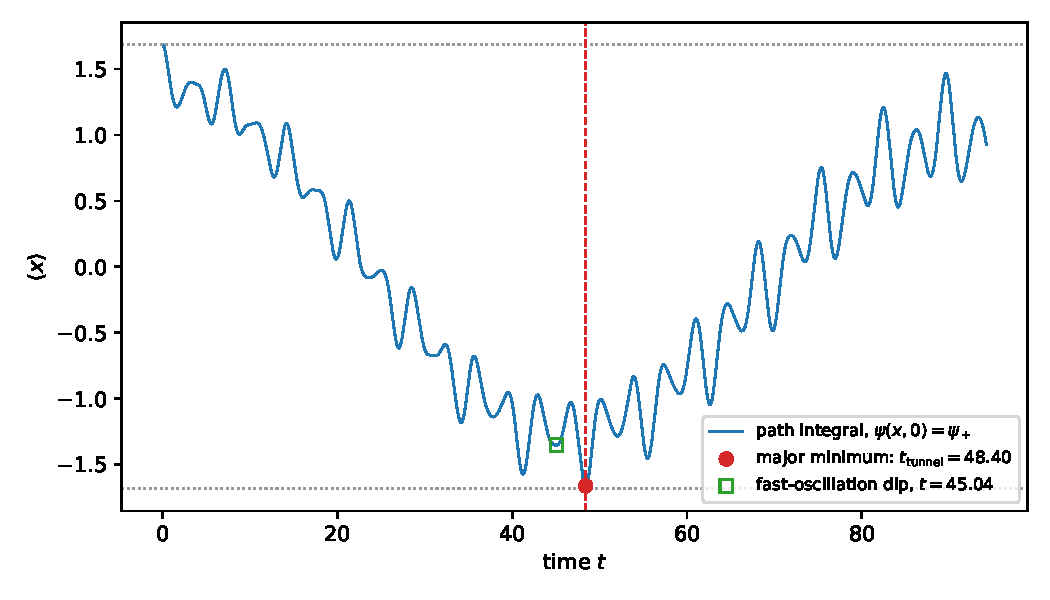
\includegraphics[width=0.7\textwidth]{figs/A_mean_x.pdf}
  \caption{$\langle x\rangle(t)$ from the path integral starting from $\psi_+$, over one full slow oscillation.}
\end{figure}

\noindent
\textbf{Major minimum:} $t_{\rm tunnel} = 48.40$, with $\langle x\rangle = -1.662$.

\noindent
\textbf{Fast fluctuation:} the smaller dips (e.g.\ $t = 45.04$, $\langle x\rangle = -1.353$) repeat every $\approx 3.6 = 2\pi/(E_2-E_1)$.
They come from the $\phi_2, \phi_3$ content of $\psi_+$ ($|\langle\phi_n|\psi_+\rangle|^2 = 0.459, 0.482, 0.039, 0.017$).
The FFT of $\langle x\rangle(t)$ has peaks at $0.067, 0.866, 1.733, 2.666$, matching $E_1-E_0,\ E_3-E_2,\ E_2-E_1,\ E_3-E_0 = 0.067, 0.845, 1.752, 2.664$.

\noindent
\textbf{Comparison with D:} D's two-state curve is a single cosine with minimum $-x_{01} = -1.477$ at $\pi/\Delta E = 47.12$.
A's curve goes deeper and its minimum is later.
Those frequency peaks at differences involving $\phi_2,\phi_3$ show that the departure from a single sinusoid is due to higher states.

\begin{lstlisting}[language=Python]
E_est, _ = lowest_states(x, dx)
T_slow = 2 * np.pi / (E_est[1] - E_est[0])
n_A = max(2048, int(np.ceil(T_slow / eps)))

K_eps = propagator(x)
psi_A = evolve(psi_well(x, x_min), K_eps, dx, n_A)
t_A = np.arange(n_A + 1) * eps
x_mean_A = mean_x(psi_A, x, dx)

t_tunnel, x_tunnel = tunnel_time(t_A, x_mean_A)
print(f"run: {n_A} steps, t_max = {t_A[-1]:.2f}  (2 pi / dE ~= {T_slow:.2f})")
print(f"t_tunnel = {t_tunnel:.4f},  <x>(t_tunnel) = {x_tunnel:.4f}")

x_mean_pi = x_mean_A[:2049:64]
\end{lstlisting}
\begin{lstlisting}[language=Python]
E6, phi6 = lowest_states(x, dx, k=6)
c = dx * phi6.T @ psi_A[0].real
print("E_n          :", np.round(E6, 5))
print("|<phi_n|psi_+>|^2:", np.round(c**2, 5))
for m, n in ((0, 1), (1, 2), (2, 3), (0, 3)):
    w = E6[n] - E6[m]
    print(f"E{n} - E{m} = {w:.4f}  ->  period {2 * np.pi / w:7.3f}")

spec = np.abs(np.fft.rfft(x_mean_A - x_mean_A.mean()))
freq = 2 * np.pi * np.fft.rfftfreq(x_mean_A.size, d=eps)
peaks = [i for i in range(1, spec.size - 1) if spec[i] > spec[i - 1] and spec[i] > spec[i + 1]]
peaks = sorted(peaks, key=lambda i: -spec[i])[:4]
print("strongest angular frequencies in <x>(t):", np.round(freq[sorted(peaks)], 3))

loc = [i for i in range(1, n_A) if x_mean_A[i] < x_mean_A[i - 1] and x_mean_A[i] < x_mean_A[i + 1]]
near = [i for i in loc if abs(t_A[i] - t_tunnel) < 12]
for i in near:
    print(f"local min  t = {t_A[i]:7.3f}  <x> = {x_mean_A[i]:+.4f}")
i_fast = max((i for i in near if t_A[i] < t_tunnel), key=lambda i: t_A[i])

w_A = np.abs(dx * phi6.T @ psi_A.T) ** 2
i_tun = int(np.argmin(x_mean_A))
for j in (0, i_tun, n_A):
    print(f"t = {t_A[j]:6.2f}: |<phi_n|psi>|^2 =", np.round(w_A[:4, j], 4))
\end{lstlisting}
\begin{lstlisting}[language=Python]
plt.figure(figsize=(7, 4))
plt.plot(t_A, x_mean_A, lw=1, label=r"path integral, $\psi(x,0)=\psi_+$")
plt.axhline(x_min, color="0.6", ls=":", lw=1)
plt.axhline(-x_min, color="0.6", ls=":", lw=1)
plt.axvline(t_tunnel, color="C3", ls="--", lw=1)
plt.plot(t_tunnel, x_tunnel, "o", color="C3",
         label=rf"major minimum: $t_{{\rm tunnel}} = {t_tunnel:.2f}$")
plt.plot(t_A[i_fast], x_mean_A[i_fast], "s", color="C2", mfc="none",
         label=rf"fast-oscillation dip, $t = {t_A[i_fast]:.2f}$")
plt.xlabel("time $t$")
plt.ylabel(r"$\langle x \rangle$")
plt.legend(fontsize=8, loc="lower right")
plt.tight_layout()
plt.savefig("figs/A_mean_x.pdf")
plt.show()
\end{lstlisting}

\section*{Problem B}
\textbf{(i) Validation} ($\lambda = \alpha/4$):
\begin{center}
\begin{tabular}{lllll}
\toprule
$\alpha$ & & Table I & $N_D = 600$ & error \\
\midrule
0.4 & $E_0$ & 1.2345071628 & 1.2344772371 & $-3.0\times10^{-5}$ \\
    & $E_1$ & 1.3469408689 & 1.3469042749 & $-3.7\times10^{-5}$ \\
0.6 & $E_0$ & 1.0624992480 & 1.0624798130 & $-1.9\times10^{-5}$ \\
    & $E_1$ & 1.4210868905 & 1.4210435761 & $-4.3\times10^{-5}$ \\
\bottomrule
\end{tabular}
\end{center}
The energies agree to 4 significant digits.
The agreement is limited by $\Delta x$: halving $\Delta x$ cuts the error by 4, the $O(\Delta x^2)$ error of the three-point formula.
Richardson extrapolation $(4E_{1200}-E_{600})/3$ then matches Table I to $4\times10^{-10}$.

\begin{lstlisting}[language=Python]
table = {0.4: (1.2345071627860, 1.3469408689225),
         0.6: (1.0624992479565, 1.4210868905393)}

x2, dx2 = make_grid(8, 1200)
for a, (E0_ref, E1_ref) in table.items():
    E_600, _ = lowest_states(x, dx, a)
    E_1200, _ = lowest_states(x2, dx2, a)
    E_rich = (4 * E_1200 - E_600) / 3
    print(f"alpha = {a}  (lambda = {a / 4:.2f})")
    for n, ref in enumerate((E0_ref, E1_ref)):
        print(f"  E{n}: table {ref:.10f}  N_D=600 {E_600[n]:.10f} (err {E_600[n] - ref:+.2e})"
              f"  N_D=1200 err {E_1200[n] - ref:+.2e}  Richardson err {E_rich[n] - ref:+.2e}")
    dE_ref = E1_ref - E0_ref
    print(f"  dE: table {dE_ref:.10f}  N_D=600 {E_600[1] - E_600[0]:.10f}"
          f" (err {E_600[1] - E_600[0] - dE_ref:+.2e})")
\end{lstlisting}

\noindent
\textbf{(ii) Convergence:}
\begin{center}
\begin{tabular}{lccccc}
\toprule
Grid & $N_D$ & $E_0$ & $E_1$ & $\Delta E$ & change in $\Delta E$ \\
\midrule
Original $[-4,4]$ & 600 & 1.27424143 & 1.34091986 & 0.06667843 & --- \\
Half spacing $[-4,4]$ & 1200 & 1.27426619 & 1.34094705 & 0.06668086 & $+2.4\times10^{-6}$ \\
Larger box $[-6,6]$ & 900 & 1.27424143 & 1.34091986 & 0.06667843 & $-1.0\times10^{-10}$ \\
\bottomrule
\end{tabular}
\end{center}
The box size has no effect; the grid spacing changes $\Delta E$ in the 6th decimal place.
I quote $E_0 = 1.2742$, $E_1 = 1.3409$ and $\Delta E = 0.06668$.
\texttt{make\_grid(L, n\_d)} sets $\Delta x = L/n_d$, and \texttt{hamiltonian(x, dx)} rebuilds $H$ for the new grid.

\begin{lstlisting}[language=Python]
E, phi = lowest_states(x, dx)
E0, E1 = E
dE = E1 - E0
print(f"original grid: E0 = {E0:.8f}, E1 = {E1:.8f}, dE = {dE:.8f}")

grids = (("Original", 8, 600), ("Half spacing", 8, 1200), ("Larger box", 12, 900))
print(f"{'grid':14s}{'L':>4s}{'N_D':>6s}{'E0':>13s}{'E1':>13s}{'dE':>13s}{'change in dE':>15s}")
for name, L, n_d in grids:
    xg, dxg = make_grid(L, n_d)
    Eg, _ = lowest_states(xg, dxg)
    dEg = Eg[1] - Eg[0]
    print(f"{name:14s}{L:4d}{n_d:6d}{Eg[0]:13.8f}{Eg[1]:13.8f}{dEg:13.8f}{dEg - dE:+15.2e}")
\end{lstlisting}

\noindent
\textbf{(iii) Eigenfunctions:}
\begin{figure}[H]
  \centering
  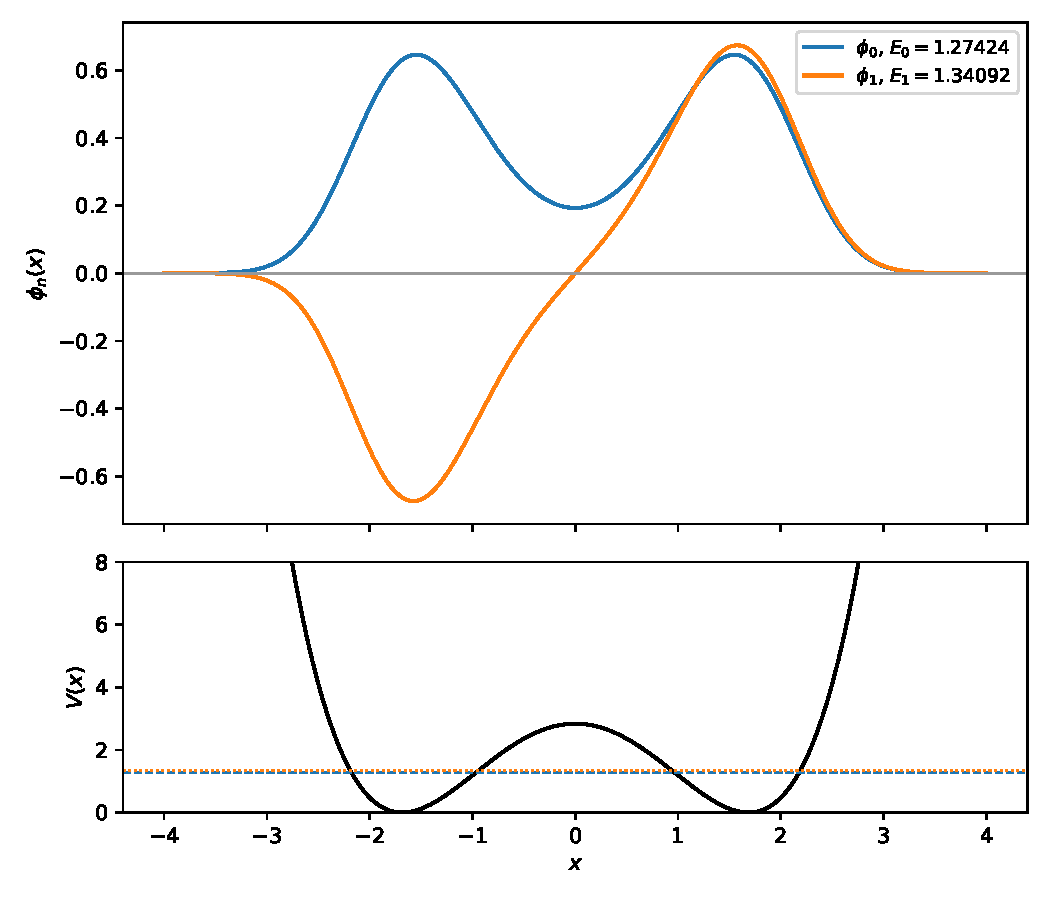
\includegraphics[width=0.65\textwidth]{figs/B_eigenfunctions.pdf}
  \caption{$\phi_0$, $\phi_1$ (top) and $V(x)$ (bottom).}
\end{figure}
\begin{lstlisting}[language=Python]
print("norms:", dx * np.sum(phi**2, axis=0))
fig, (ax1, ax2) = plt.subplots(2, 1, figsize=(7, 6), sharex=True,
                               gridspec_kw={"height_ratios": [2, 1]})
ax1.plot(x, phi[:, 0], label=rf"$\phi_0$, $E_0 = {E0:.5f}$")
ax1.plot(x, phi[:, 1], label=rf"$\phi_1$, $E_1 = {E1:.5f}$")
ax1.axhline(0, color="0.6", lw=0.8)
ax1.set_ylabel(r"$\phi_n(x)$")
ax1.legend(fontsize=9)
ax2.plot(x, V(x), "k")
ax2.axhline(E0, color="C0", ls="--", lw=1)
ax2.axhline(E1, color="C1", ls=":", lw=1)
ax2.set_ylim(0, 8)
ax2.set_xlabel("$x$")
ax2.set_ylabel("$V(x)$")
plt.tight_layout()
plt.savefig("figs/B_eigenfunctions.pdf")
plt.show()
\end{lstlisting}

\section*{Problem C}
\textbf{(i) Energies:}
\begin{center}
\begin{tabular}{lcccc}
\toprule
 & harmonic & numerical & signed error & relative error \\
\midrule
$E_{\rm S}$ vs $E_0$ & 1.444086 & 1.274241 & $+0.1698$ & 0.133 \\
$E_{\rm A}$ vs $E_1$ & 1.450345 & 1.340920 & $+0.1094$ & 0.082 \\
gap & 0.006259 & 0.066678 & $-0.0604$ & 0.906 \\
\bottomrule
\end{tabular}
\end{center}
The gap error is $(E_{\rm A}-E_1)-(E_{\rm S}-E_0) = 0.1094-0.1698 = -0.0604$.
The energies are more accurate in relative terms than the gap.

\begin{lstlisting}[language=Python]
H = hamiltonian(x, dx)
psi_p, psi_m = psi_well(x, x_min), psi_well(x, -x_min)
psi_S = (psi_p + psi_m) / np.sqrt(2)
psi_Anti = (psi_p - psi_m) / np.sqrt(2)

def energy(psi):
    return (dx * psi @ (H @ psi)) / (dx * psi @ psi)

E_S, E_A = energy(psi_S), energy(psi_Anti)
print(f"overlap <psi_+|psi_-> = {dx * psi_p @ psi_m:.3e}")
print(f"norms: <S|S> = {dx * psi_S @ psi_S:.6f}, <A|A> = {dx * psi_Anti @ psi_Anti:.6f}")
for name, Eh, En in (("E_S vs E0", E_S, E0), ("E_A vs E1", E_A, E1), ("gap", E_A - E_S, dE)):
    print(f"{name:10s}: harmonic {Eh:.6f}  numerical {En:.6f}  "
          f"signed err {Eh - En:+.6f}  rel err {abs(Eh - En) / abs(En):.4f}")
\end{lstlisting}

\noindent
\textbf{(ii) Wave functions:}
\begin{figure}[H]
  \centering
  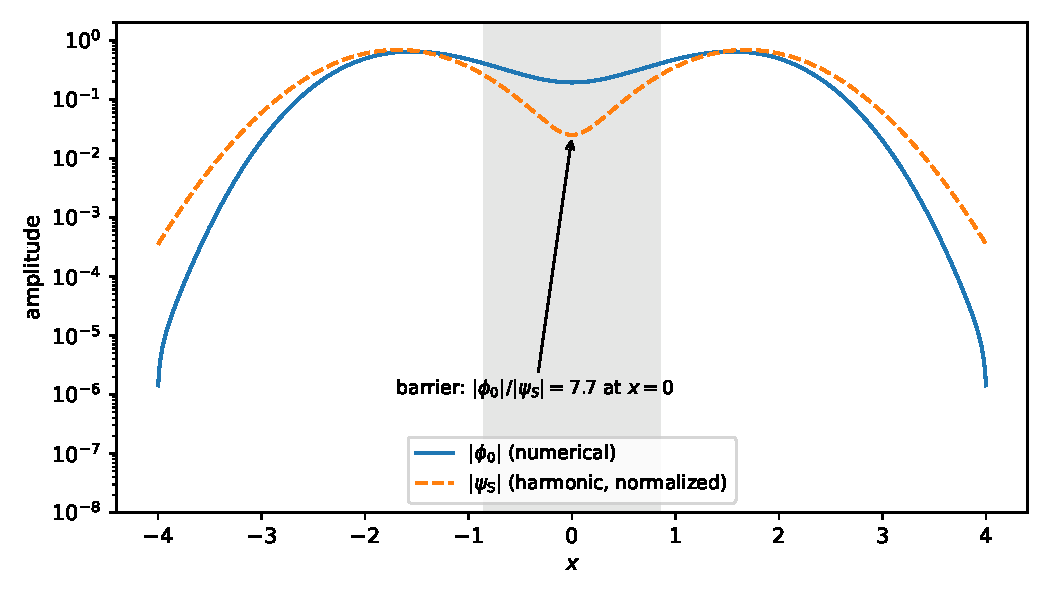
\includegraphics[width=0.7\textwidth]{figs/C_log_psi.pdf}
  \caption{$|\phi_0|$ and normalized $|\psi_{\rm S}|$, log scale. Shaded: barrier region.}
\end{figure}
\noindent
At $x = 0$, $|\phi_0|$ is $7.7$ times larger than $|\psi_{\rm S}|$.
The harmonic wells give a barrier $V_+(0) = 4/\alpha = 11.35$, much higher than the true $V(0) = 1/\alpha = 2.84$, so $\psi_{\rm S}$ decays too fast under the barrier.
This underestimates the tunneling, so the gap comes out $\sim10\times$ too small.
The energy errors ($0.17$ and $0.11$) are each larger than the gap ($0.067$), and their difference ($0.06$) is almost the size of the gap.
That is why a 8--13\% error in the energies becomes a 91\% error in the gap.

\begin{lstlisting}[language=Python]
psi_S_n = psi_S / np.sqrt(dx * psi_S @ psi_S)
i0 = N_D // 2   # x[300] = 0
print(f"V(0) = {V(0.0):.4f},  V_+(0) = 4 x_min^2 = {4 * x_min**2:.4f}")
print(f"at x = 0: |psi_S| = {abs(psi_S_n[i0]):.3e},  |phi_0| = {abs(phi[i0, 0]):.3e},"
      f"  ratio phi_0/psi_S = {abs(phi[i0, 0] / psi_S_n[i0]):.1f}")

plt.figure(figsize=(7, 4))
plt.semilogy(x, np.abs(phi[:, 0]), label=r"$|\phi_0|$ (numerical)")
plt.semilogy(x, np.abs(psi_S_n), "--", label=r"$|\psi_{\rm S}|$ (harmonic, normalized)")
plt.annotate(f"barrier: $|\\phi_0|/|\\psi_S| = {abs(phi[i0, 0] / psi_S_n[i0]):.1f}$ at $x=0$",
             xy=(0, abs(psi_S_n[i0])), xytext=(-1.7, 1e-6), fontsize=9,
             arrowprops=dict(arrowstyle="->"))
plt.axvspan(-0.5 * x_min, 0.5 * x_min, color="0.9")
plt.ylim(1e-8, 2)
plt.xlabel("$x$")
plt.ylabel("amplitude")
plt.legend(fontsize=9, loc="lower center")
plt.tight_layout()
plt.savefig("figs/C_log_psi.pdf")
plt.show()
\end{lstlisting}

\section*{Problem D}
\textbf{(i)} With real $\phi_0,\phi_1$,
\[
  |\psi|^2 = \tfrac12\left[\phi_0^2 + \phi_1^2 + 2\phi_0\phi_1\cos(\Delta E\,t/\hbar)\right].
\]
Normalization ($\int\phi_n\phi_m\,dx = \delta_{nm}$) gives $\int|\psi|^2dx = 1$, so no denominator is needed.
Symmetry ($\phi_0$ even, $\phi_1$ odd) gives $\int x\phi_0^2\,dx = \int x\phi_1^2\,dx = 0$.
Hence
\[
  \langle x\rangle = x_{01}\cos(\Delta E\,t/\hbar),
\]
with $x_{01} = 1.477 > 0$ for B's signs.
$\langle x\rangle$ is first at its minimum when $\Delta E\,t/\hbar = \pi$, i.e.\ $t_{\rm tunnel} = \pi\hbar/\Delta E = 47.12$.

\noindent
\textbf{(ii)} $T = 2\pi/\Delta E = 94.23$; I evolved 3840 steps, to $t = 94.25$.

\noindent
\textbf{(iii)}
\begin{figure}[H]
  \centering
  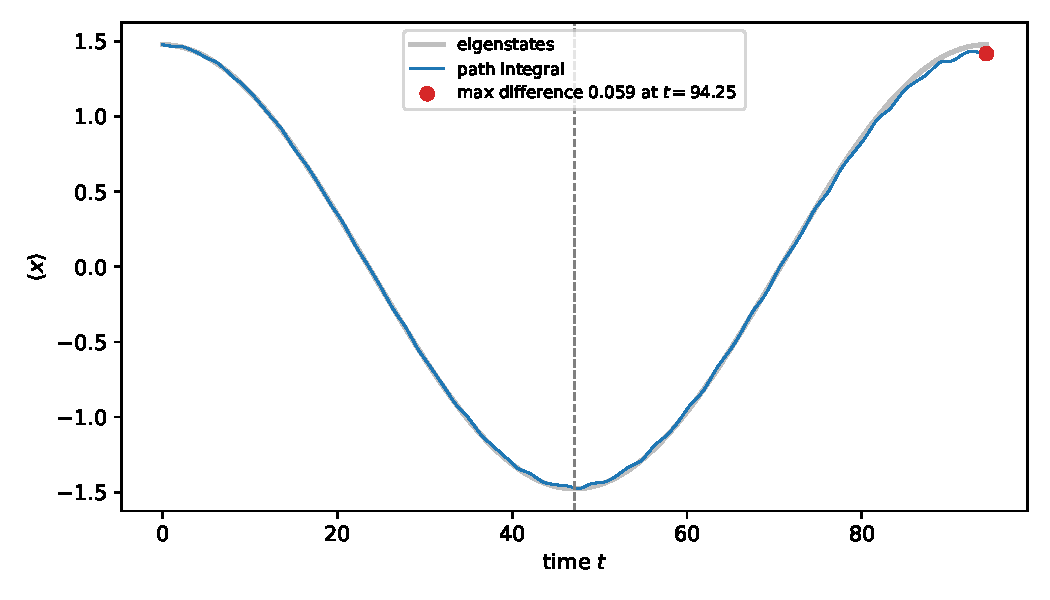
\includegraphics[width=0.7\textwidth]{figs/D_mean_x.pdf}
  \caption{$\langle x\rangle(t)$ from the eigenstates and the path integral.}
\end{figure}
\begin{figure}[H]
  \centering
  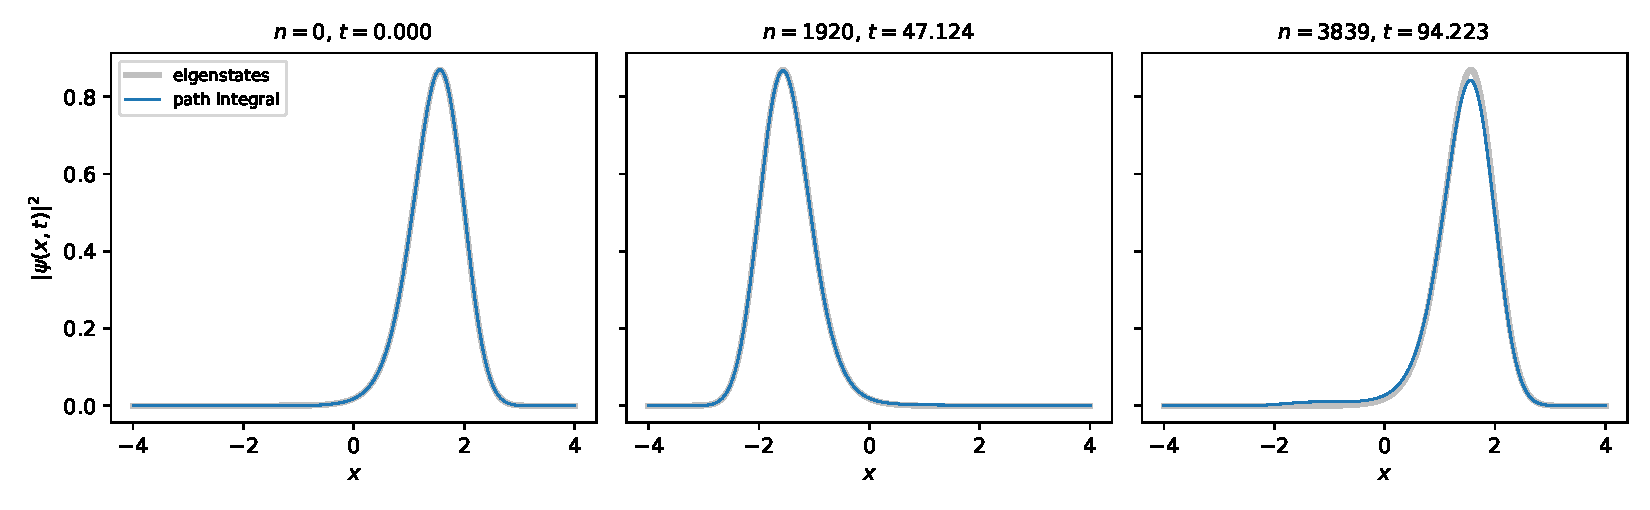
\includegraphics[width=\textwidth]{figs/D_densities.pdf}
  \caption{$|\psi(x,t)|^2$ from both methods at the steps nearest $0$, $t_{\rm tunnel}$, and $T$.}
\end{figure}
\noindent
The maximum difference is $\max|\langle x\rangle_{\rm PI}-\langle x\rangle_{\rm eig}| = 0.0595$, at $t = 94.25$: $\langle x\rangle_{\rm PI} = 1.4175$, $\langle x\rangle_{\rm eig} = 1.4770$.

\noindent
\textbf{Pattern:} the PI amplitude decays slowly; the difference is $0.006$ at $T/2$ and $0.06$ at $T$.

\noindent
\textbf{Possible cause:} $\Delta x\,\tilde{\mathcal K}$ is not unitary and damps $\phi_1$ slightly more than $\phi_0$ each step.
Renormalizing then shifts weight toward $\phi_0$.

\noindent
\textbf{Check and prediction:} track $w_n = |\langle\phi_n|\psi_{\rm PI}\rangle|^2$.
If this is the cause, $w_0/w_1$ drifts away from $0.5/0.5$ while $w_0+w_1 \approx 1$.
(I ran it: $0.624/0.376$ at $T$.)

\begin{lstlisting}[language=Python]
T = 2 * np.pi / dE
n_D = int(np.ceil(T / eps))
t_D = np.arange(n_D + 1) * eps
psi0_D = (phi[:, 0] + phi[:, 1]) / np.sqrt(2)

x01 = dx * np.sum(phi[:, 0] * x * phi[:, 1])
psi_eig = (np.exp(-1j * E0 * t_D)[:, None] * phi[:, 0]
           + np.exp(-1j * E1 * t_D)[:, None] * phi[:, 1]) / np.sqrt(2)
x_eig = mean_x(psi_eig, x, dx)
print(f"x01 = {x01:.6f};  max |grid <x> - x01 cos(dE t)| = {np.abs(x_eig - x01 * np.cos(dE * t_D)).max():.1e}")

x_mean_eig = x01 * np.cos(dE * np.arange(0, 2049, 64) * eps)

psi_PI = evolve(psi0_D.astype(np.complex128), K_eps, dx, n_D)
x_PI = mean_x(psi_PI, x, dx)

diff = np.abs(x_PI - x_eig)
n_max = np.argmax(diff)
print(f"T = {T:.4f}, n_D = {n_D}, t_last = {t_D[-1]:.4f}")
print(f"max |<x>_PI - <x>_eig| = {diff[n_max]:.4f} at t = {t_D[n_max]:.4f}: "
      f"PI {x_PI[n_max]:+.4f}, eig {x_eig[n_max]:+.4f}")
for f in (0.25, 0.5, 0.75, 1.0):
    j = int(round(f * n_D))
    print(f"  t = {t_D[j]:7.3f}: PI {x_PI[j]:+.4f}  eig {x_eig[j]:+.4f}  diff {x_PI[j] - x_eig[j]:+.4f}")
print(f"min of PI curve: t = {t_D[np.argmin(x_PI)]:.4f};  pi/dE = {np.pi / dE:.4f}")
\end{lstlisting}
\begin{lstlisting}[language=Python]
fig, ax = plt.subplots(figsize=(7, 4))
ax.plot(t_D, x_eig, lw=2, color="0.75", label="eigenstates")
ax.plot(t_D, x_PI, "C0", lw=1, label="path integral")
ax.plot(t_D[n_max], x_PI[n_max], "o", color="C3",
        label=rf"max difference ${diff[n_max]:.3f}$ at $t = {t_D[n_max]:.2f}$")
ax.axvline(np.pi / dE, color="0.5", ls="--", lw=1)
ax.set_xlabel("time $t$")
ax.set_ylabel(r"$\langle x \rangle$")
ax.legend(fontsize=8, loc="upper center")
plt.tight_layout()
plt.savefig("figs/D_mean_x.pdf")
plt.show()

fig, axes = plt.subplots(1, 3, figsize=(11, 3.4), sharey=True)
for ax, t_target in zip(axes, (0.0, np.pi / dE, T)):
    j = int(np.argmin(np.abs(t_D - t_target)))
    ax.plot(x, np.abs(psi_eig[j]) ** 2, lw=2.5, color="0.75", label="eigenstates")
    ax.plot(x, np.abs(psi_PI[j]) ** 2, "C0", lw=1, label="path integral")
    ax.set_title(f"$n = {j}$, $t = {t_D[j]:.3f}$", fontsize=10)
    ax.set_xlabel("$x$")
axes[0].set_ylabel(r"$|\psi(x,t)|^2$")
axes[0].legend(fontsize=8)
plt.tight_layout()
plt.savefig("figs/D_densities.pdf")
plt.show()
\end{lstlisting}
\begin{lstlisting}[language=Python]
w_PI = np.abs(dx * phi.T @ psi_PI.T) ** 2
for j in (0, n_D // 2, n_D):
    print(f"t = {t_D[j]:7.3f}: w0 = {w_PI[0, j]:.4f}, w1 = {w_PI[1, j]:.4f}, "
          f"w0 + w1 = {w_PI[:, j].sum():.4f}, 2 sqrt(w0 w1) x01 = {2 * np.sqrt(w_PI[0, j] * w_PI[1, j]) * x01:.4f}")
\end{lstlisting}

\section*{Problem E (bonus)}
\begin{center}
\begin{tabular}{cccccc}
\toprule
$\alpha$ & $\Delta E$ & $\pi/\Delta E$ & $t_{\rm tunnel}$ & $t_{\rm tunnel}\Delta E/\pi$ & two-state fraction \\
\midrule
0.30 & 0.029872 & 105.17 & 100.04 & 0.951 & 0.954 \\
0.35 & 0.064656 & 48.59 & 48.40 & 0.996 & 0.942 \\
0.40 & 0.112427 & 27.94 & 28.15 & 1.008 & 0.930 \\
0.45 & 0.169294 & 18.56 & 17.75 & 0.956 & 0.921 \\
0.50 & 0.231199 & 13.59 & 13.52 & 0.995 & 0.913 \\
\bottomrule
\end{tabular}
\end{center}
\begin{figure}[H]
  \centering
  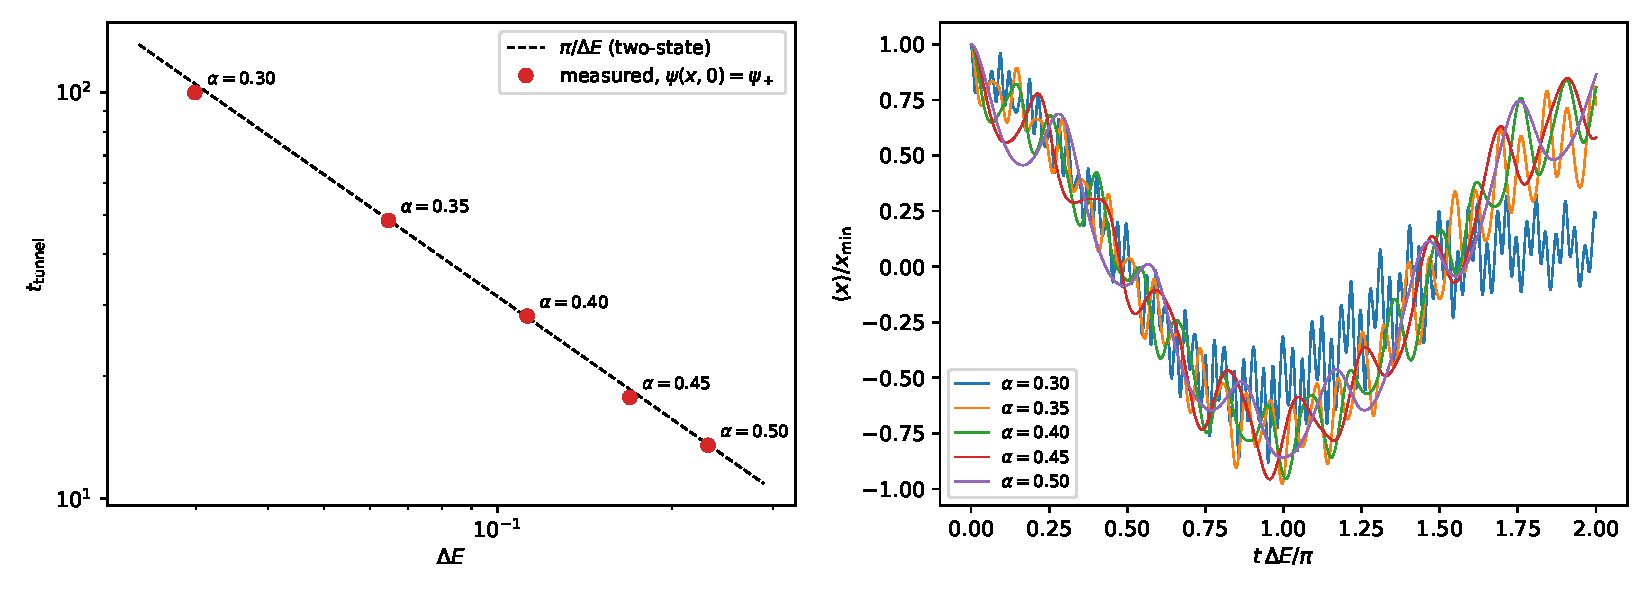
\includegraphics[width=\textwidth]{figs/E_tunnel.pdf}
  \caption{Left: $t_{\rm tunnel}$ vs $\Delta E$ with $\pi/\Delta E$. Right: $\langle x\rangle/x_{\min}$ vs $t\Delta E/\pi$.}
\end{figure}
\noindent
The prediction holds to within 5\%.
The deviations do not follow the two-state fraction: $\alpha = 0.50$ has the smallest fraction ($0.913$) but agrees to $0.5\%$, while $\alpha = 0.30$ has the largest ($0.954$) but is off by $5\%$.
The higher states cause the fast oscillation (period $\approx 3.5$), which makes the minimum uncertain by about half a period.
For $\alpha = 0.30$, the long run also lets numerical error build up: the two-state weight of the evolved state drops to $0.66$ by $t_{\rm tunnel}$.
So the results support higher states as the source of the fast oscillation, but not of the deviation from $\pi/\Delta E$.

\begin{lstlisting}[language=Python]
alpha_list = [0.30, 0.35, 0.40, 0.45, 0.50]
delta_E_list, t_tunnel_list, frac_list, frac_tun, fast_rms, curves = [], [], [], [], [], []
for a in alpha_list:
    Ea, phia = lowest_states(x, dx, a, k=3)
    dEa = Ea[1] - Ea[0]
    xm_a = 1 / np.sqrt(a)
    pp = psi_well(x, xm_a)
    pp = pp / np.sqrt(dx * pp @ pp)
    n_a = int(np.ceil(2 * np.pi / dEa / eps))
    psi_a = evolve(pp, propagator(x, a), dx, n_a)
    xs = mean_x(psi_a, x, dx)
    ts = np.arange(n_a + 1) * eps
    t_tun, _ = tunnel_time(ts, xs)
    frac_tun.append(np.sum(np.abs(dx * phia[:, :2].T @ psi_a[np.argmin(xs)]) ** 2))
    win = int(round(2 * np.pi / (Ea[2] - Ea[1]) / eps))
    smooth = np.convolve(xs, np.ones(win) / win, mode="same")
    core = slice(win, n_a + 1 - win)
    delta_E_list.append(dEa)
    t_tunnel_list.append(t_tun)
    frac_list.append(np.sum((dx * phia[:, :2].T @ pp) ** 2))
    fast_rms.append(np.sqrt(np.mean((xs - smooth)[core] ** 2)))
    curves.append((ts, xs))
    print(f"alpha = {a:.2f}: dE = {dEa:.6f}, pi/dE = {np.pi / dEa:8.3f}, t_tunnel = {t_tun:8.3f}, "
          f"ratio = {t_tun * dEa / np.pi:.4f}, two-state fraction = {frac_list[-1]:.4f} "
          f"(at t_tunnel: {frac_tun[-1]:.4f}), "
          f"fast rms = {fast_rms[-1]:.3f}, fast period = {2 * np.pi / (Ea[2] - Ea[1]):.2f}")
\end{lstlisting}
\begin{lstlisting}[language=Python]
dE_arr = np.array(delta_E_list)
fig, (ax1, ax2) = plt.subplots(1, 2, figsize=(11, 4))
grid_dE = np.geomspace(dE_arr.min() * 0.8, dE_arr.max() * 1.25, 50)
ax1.loglog(grid_dE, np.pi / grid_dE, "k--", lw=1, label=r"$\pi/\Delta E$ (two-state)")
ax1.loglog(dE_arr, t_tunnel_list, "o", color="C3", label=r"measured, $\psi(x,0)=\psi_+$")
for a, dEa, tt in zip(alpha_list, dE_arr, t_tunnel_list):
    ax1.annotate(rf"$\alpha={a:.2f}$", (dEa, tt), textcoords="offset points", xytext=(6, 4), fontsize=8)
ax1.set_xlabel(r"$\Delta E$")
ax1.set_ylabel(r"$t_{\rm tunnel}$")
ax1.legend(fontsize=9)
for a, dEa, (ts, xs) in zip(alpha_list, dE_arr, curves):
    ax2.plot(ts * dEa / np.pi, xs * np.sqrt(a), lw=0.8, label=rf"$\alpha={a:.2f}$")
ax2.set_xlabel(r"$t\,\Delta E/\pi$")
ax2.set_ylabel(r"$\langle x\rangle / x_{\min}$")
ax2.legend(fontsize=8)
plt.tight_layout()
plt.savefig("figs/E_tunnel.pdf")
plt.show()
\end{lstlisting}

\section*{results.json}
\begin{lstlisting}[language=Python]
results = {
    "tsn": TSN,
    "alpha": alpha,
    "x_mean_pi": x_mean_pi.tolist(),
    "t_tunnel": float(t_tunnel),
    "E0": float(E0), "E1": float(E1),
    "phi0": phi[:, 0].tolist(), "phi1": phi[:, 1].tolist(),
    "E_S": float(E_S), "E_A": float(E_A),
    "x_mean_eig": x_mean_eig.tolist(),
    "delta_E_list": [float(dE) for dE in delta_E_list],
    "t_tunnel_list": [float(t) for t in t_tunnel_list],
}
with open("results.json", "w") as f:
    json.dump(results, f)
print({k: (len(v) if isinstance(v, list) else v) for k, v in results.items()})
\end{lstlisting}

\section*{AI use appendix}
I used an AI assistant (Claude, Anthropic) only for debugging.
When my code raised errors or gave unexpected output, I showed the relevant code and error messages to the assistant and asked it to help locate the cause.
I then checked each suggested fix myself before applying it.
\textbf{What it got wrong and how I caught it:} TODO.

\end{document}
